\chapter{Microservizio anagrafica}\label{cap:microservizio-anagrafica}

\section{Scopo del sistema}

Il sistema di anagrafica si occupa di gestire le informazioni anagrafiche dei sensori, delle aree e dei lampioni. Gestisce questi raggruppamenti e si occupa di renderli persistenti su database.

\section{Requisiti coperti dal sistema}

\subsection{RF\_03}
RF\_03:deve essere possibile aggiungere nuovi sensori a sistema.

Questo microservizio, copre il requisito peristendo i dati anagrafici del sensore.

\subsection{RF\_08}
RF\_08:l'utente deve poter inserire la locazione geografica del sensore nel sistema.

Questo microservizio, copre il requisito peristendo i dati di locazione del sensore.

\subsection{RF\_09}
RF\_09:l'utente deve poter inserire il raggio di azione del sensore.

Questo microservizio, copre il requisito peristendo i dati di raggio di azione del sensore.

\subsection{RF\_10}
RF\_10:l'utente deve poter essere in grado di visualizzare quali aree sono illuminate in un dato momento

Questo microservizio, copre parte del requisito fornendo l'informazione di quali lampioni si trovano in una determinata area.



\section{Descrizione del sistema}

Il sistema principalmente fornisce le informazioni stoccate su base dati tramite un'interfaccia rest.
Questo è poi in grado di fornire i dati in forma aggregata, come ad esempio il numero di lampioni per area, o il numero di sensori per lampioni.

Per queste informazioni ha inoltre il compito e la responsabilità di tenere aggiornati i dati nel database.

\section{Architettura del sistema}

L'architettura base del sistema è in MVVM perché non è presente la necessità di multi input e multi output e un'architettura di altro tipo avrebbe aggiunto complessità inutile al sistema.

I componenti del programma sono quindi divisi in tre parti: Model, View e ViewModel.

\begin{figure}[h]
    \centering
    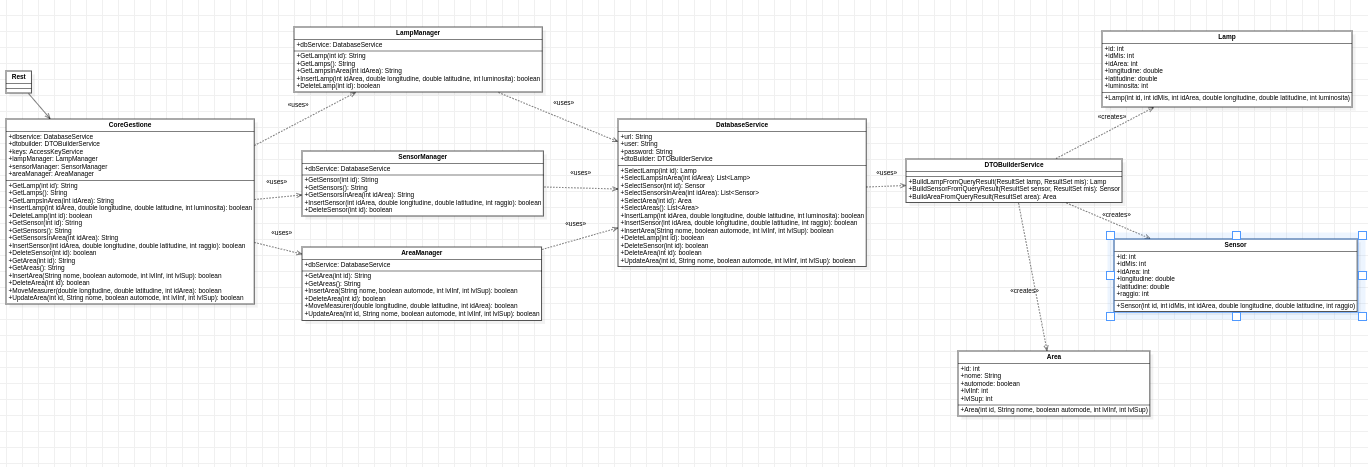
\includegraphics[width=\textwidth]{img/anagrafe_generale.png}
    \caption{Vista generale del sistema di anagrafe}
    \label{fig:general_anagrafe}
\end{figure}

\section{Model}
\begin{figure}[h]
    \centering
    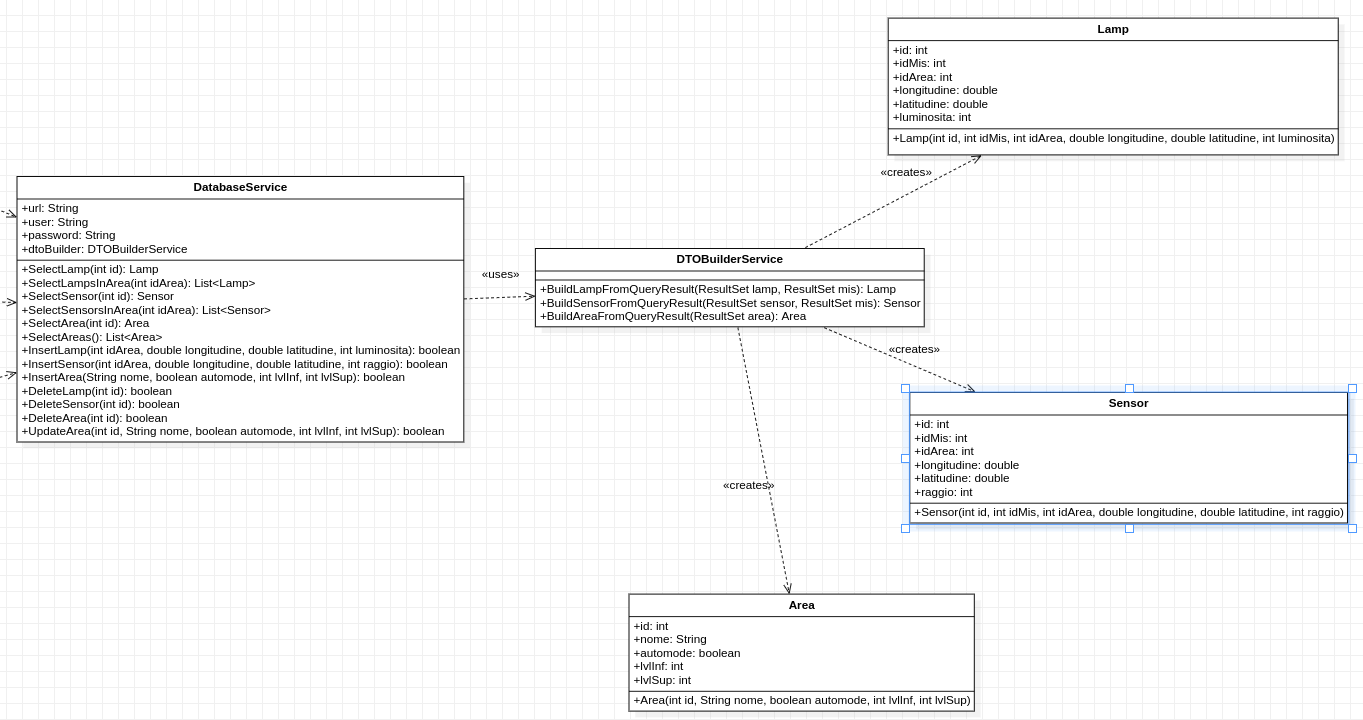
\includegraphics[width=\textwidth]{img/model_anagrafe.png}
    \caption{Diagramma delle classi del modello all'interno del sistema di anagrafe}
    \label{fig:model_anagrafe}
\end{figure}

\section{ViewModel}

\section{View}


